\documentclass{article}
\usepackage{graphicx}
\usepackage[margin=1.5cm]{geometry}
\usepackage{amsmath}

\begin{document}
\twocolumn

\title{Wednesday Warm Up: Unit 3, Magnetic Forces and Fields}
\author{Prof. Jordan C. Hanson}

\maketitle

\section{Memory Bank}

\begin{itemize}
\item $\hat{i} \times \hat{j} = \hat{k}$, $\hat{j} \times \hat{k} = \hat{i}$, $\hat{k} \times \hat{i} = \hat{j}$ ... The direction of the \textit{cross-product} follows this pattern.  Reversing the order of any two vectors introduces a minus sign.
\item $\hat{i} \times \hat{i} = 0$, $\hat{j} \times \hat{j} = 0$, $\hat{k} \times \hat{k} = 0$ ... The \textit{cross-product} is zero when both vectors are parallel.
\item $|\vec{a} \times \vec{b}| = |\vec{a}||\vec{b}|\sin\theta$ ... The magnitude of the cross-product of two vectors $\vec{a}$ and $\vec{b}$, given the angle $\theta$ between them.
\item $\vec{F} = I\vec{L} \times \vec{B}$ ... The Lorentz force, by a magnetic field $\vec{B}$ on a \textit{current} $i$ of length and direction $\vec{L}$.
\item $\vec{F} = q\vec{v} \times \vec{B}$ ... The Lorentz force, by a magnetic field $\vec{B}$ on a \textit{charge} $q$ with velocity $\vec{v}$.
\end{itemize}

\section{The Cross-Product}

\begin{enumerate}
\item Let $\vec{a} = 2\hat{i}-1\hat{j}$, and $\vec{b} = 4\hat{i}-2\hat{j}$.  Calculate $\vec{a} \times \vec{b}$.  What is the angle between the two vectors?  \\ \vspace{1cm}
\end{enumerate}

\section{Magnetic Force on Currents and Charge}

\begin{enumerate}
\item A cosmic ray electron moves at $7.50 \times 10^6$ m s$^{-1}$ perpendicular to the magnetic field of the Earth at an altitude where field strength is $1.00\times 10^{-5}$ T.  What is the radius of the circular path the electron follows? \\ \vspace{3cm}
\item (a) An oxygen-16 ion with a mass of $2.66\times 10^{-26}$ kg travels at $5.00\times 10^6$ m s$^{-1}$ perpendicular to a $1.20$ T magnetic field, which makes it move in a circular arc with a 0.231 m radius. What positive charge is on the ion? (b) What is the ratio of this charge to the charge of an electron? (c) Discuss why the ratio found in (b) should be an integer. \\ \vspace{4cm}
\item Consider Fig. \ref{fig:2}, in which a \textit{tokamak} is shown.  Tokamaks are systems designed to contain a plasma for fusion reactions.  (a) Use the right hand rule to show that the solenoidal B-field that we have measured becomes \textit{toroidal}, given the geometry of the external current. (b) The solenoidal and toroidal B-fields originate from Amp\`{e}re's Law, which states that a current creates a B-field that circles around it.  If positive ions in the plasma are circling as shown in Fig. \ref{fig:2}, show that they produce a poloidal B-field, as shown. (c) Convince yourself that the sum of the toroidal and poloidal B-fields forms the corkscrew pattern shown in Fig. \ref{fig:2}.
\end{enumerate}

\begin{figure}
\centering
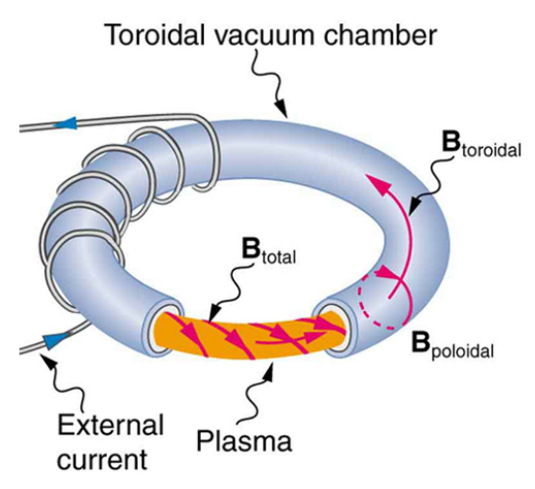
\includegraphics[width=0.35\textwidth]{figures/tokamak.png}
\caption{\label{fig:2} This structure is called a \textit{tokamak}, and it is used to confine plasma in a fusion reactor.}
\end{figure}

\end{document}
